\documentclass[aspectratio=169]{beamer}
\usepackage{color,amsmath}
\usepackage{subfigure}
\usepackage{booktabs}
\usepackage{framed}
\usepackage{comment}
\usepackage{hyperref}
\hypersetup{
    colorlinks=true,
    linkcolor=blue
}
\usepackage{ulem}

%%%%%%%%%%%%%%%%%%%%%%%%%%
\title[]{Introduction to mass collaboration}
\author[]{Matthew J. Salganik\\Department of Sociology\\Princeton University}
\date[]{Summer Institutes in Computational Social Science\\2020
\vfill
\begin{flushleft}
{\scriptsize
The Summer Institutes in Computational Social Science is supported by grants from the Russell Sage Foundation and the Alfred P. Sloan Foundation.}
\end{flushleft}
\begin{flushright}

\includegraphics[width=0.1\textwidth]{figures/cc-by.png}
\end{flushright}
}
\begin{document}
%%%%%%%%%%%%%%%%%%%%%%%%%%
\frame{\titlepage}
%%%%%%%%%%%%%%%%%%%%%%%%%%
\begin{frame}

Schedule: \url{https://compsocialscience.github.io/summer-institute/2019/\#schedule}

\end{frame}
%%%%%%%%%%%%%%%%%%%%%%%%%%%
\begin{frame}

\begin{itemize}
\item Observing behavior
\item Asking questions
\item Running experiments
\item \textcolor{blue}{Creating mass collaboration}
\end{itemize}

\end{frame}
%%%%%%%%%%%%%%%%%%%%%%%%%%%
\begin{frame}

\begin{center}

\includegraphics[width=0.5\textwidth]{figures/wikipedia_logo}
\end{center}

\end{frame}
%%%%%%%%%%%%%%%%%%%%%%%%%%
\begin{frame}

Mass collaboration combines ideas from 
\begin{itemize}
\item crowdsourcing
\item citizen science
\item collective intelligence
\end{itemize}

\end{frame}
%%%%%%%%%%%%%%%%%%%%%%%%%%%
\begin{frame}

\begin{center}
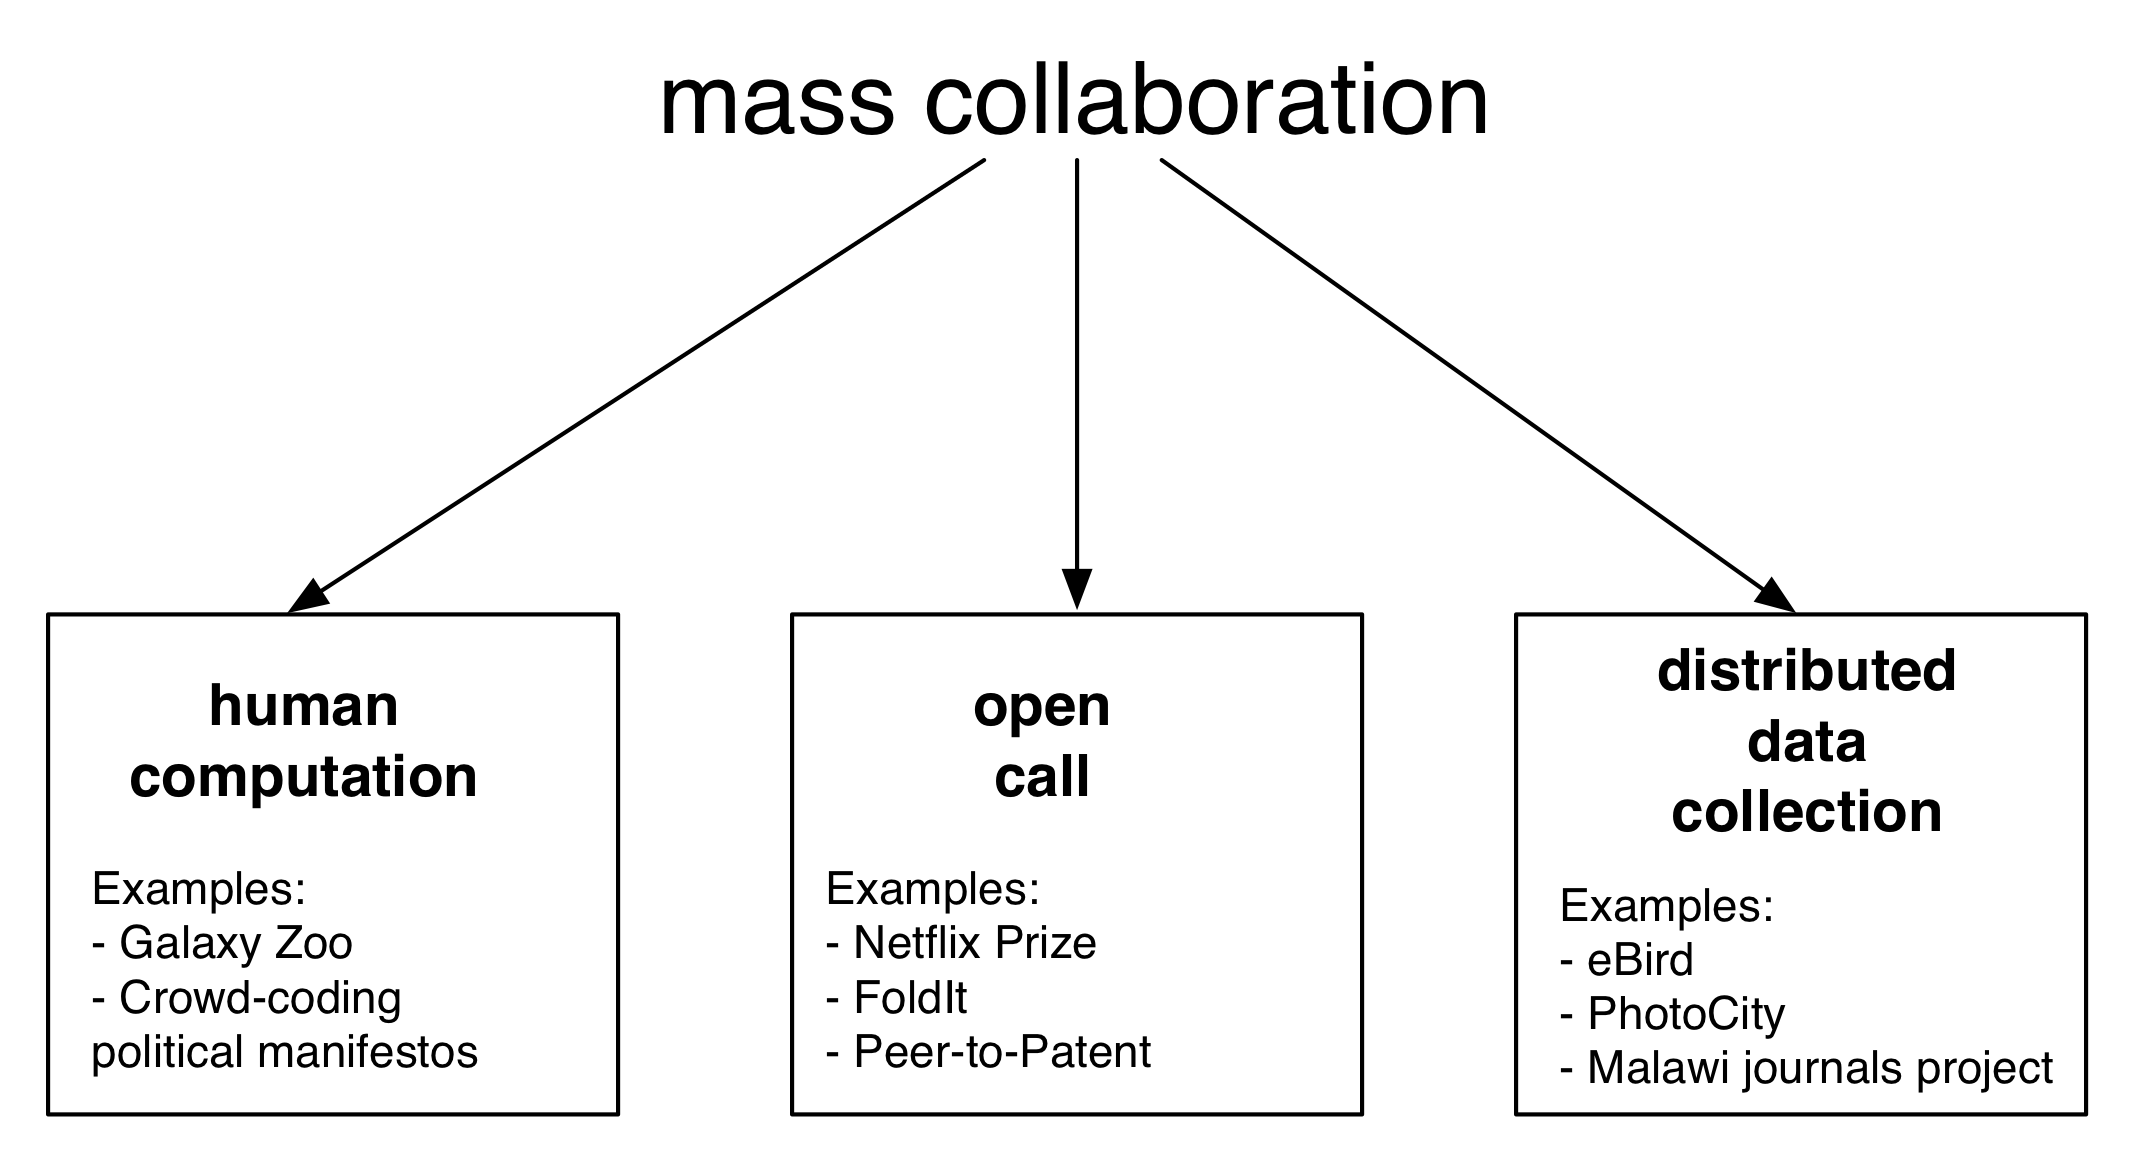
\includegraphics[width=\textwidth]{figures/mass_collaboration_schematic}
\end{center}

\end{frame}
%%%%%%%%%%%%%%%%%%%%%%%%%%
\begin{frame}

Guiding idea:\\
Collaborators not cogs (ornithology and astronomy are examples)

\end{frame}
%%%%%%%%%%%%%%%%%%%%%%%%%%
\begin{frame}

\begin{itemize}
\item Is this really research?
\pause 
\item Does this enable new research?
\end{itemize}

\end{frame}
%%%%%%%%%%%%%%%%%%%%%%%%%%
\begin{frame}

\begin{itemize}
\item Is this perfect?
\pause
\item Is this better than we can do without mass collaboration?
\end{itemize}

\end{frame}
%%%%%%%%%%%%%%%%%%%%%%%%%%
\begin{frame}

\begin{itemize}
\item Is this impossible?
\pause
\item Is this possible?
\end{itemize}

\end{frame}
%%%%%%%%%%%%%%%%%%%%%%%%%%
\begin{frame}

An honest assessment: \pause As far as I can tell, most mass collaborations fail

\end{frame}
%%%%%%%%%%%%%%%%%%%%%%%%%%
\begin{frame}

\begin{itemize}
\item \textcolor{blue}{Human computation}
\item Open call
\item Distributed data collection
\end{itemize}

\end{frame}
%%%%%%%%%%%%%%%%%%%
\begin{frame}

\begin{itemize}
\item Easy task, big scale
\pause
\item Humans better than computers
\pause
\item Can be combined with supervised learning 
\pause
\item Increasingly important as we move from numeric survey data to working with text, images, movies, audio, etc.
\end{itemize}

\end{frame}
%%%%%%%%%%%%%%%%%%%%%%%%%%
\begin{frame}

\begin{center}
\only<1>{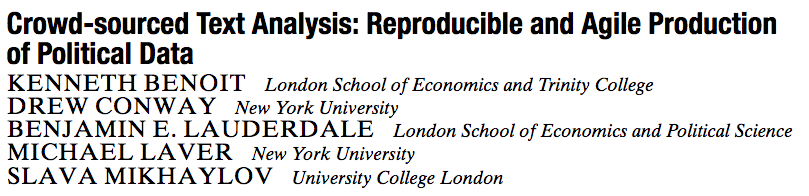
\includegraphics[width=\textwidth]{figures/benoit_crowd-sourced_2016_title}}
\only<2>{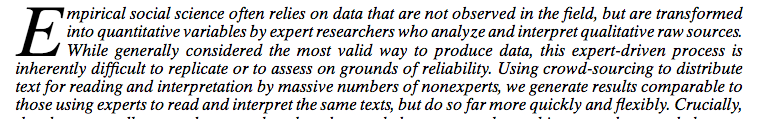
\includegraphics[width=\textwidth]{figures/benoit_crowd-sourced_2016_abstract}}
\end{center}

\vfill
{\tiny \url{http://dx.doi.org/10.1017/S0003055416000058}}

\end{frame}
%%%%%%%%%%%%%%%%%%%%%%%%%%
\begin{frame}

Here's a piece of the manifesto of the Labor Party in the United Kingdom from 2010:

\begin{quote}
``Millions of people working in our public services embody the best values of Britain, helping empower people to make the most of their own lives while protecting them from the risks they should not have to bear on their own. Just as we need to be bolder about the role of government in making markets work fairly, we also need to be bold reformers of government.''
\end{quote}

\end{frame}
%%%%%%%%%%%%%%%%%%%%%%%%%%
\begin{frame}

\begin{center}
\only<1>{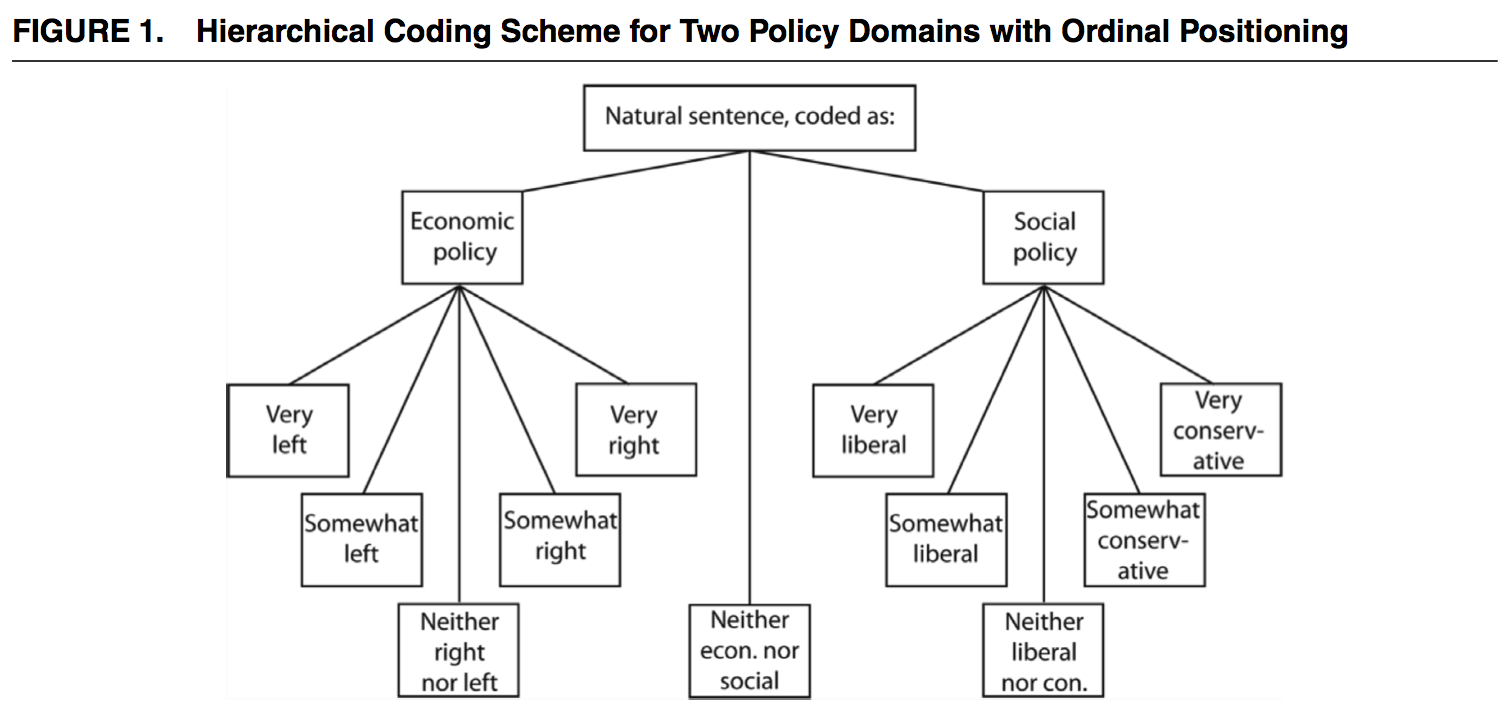
\includegraphics[width=\textwidth]{figures/benoit_crowd-sourced_2016_fig1}}
\only<2>{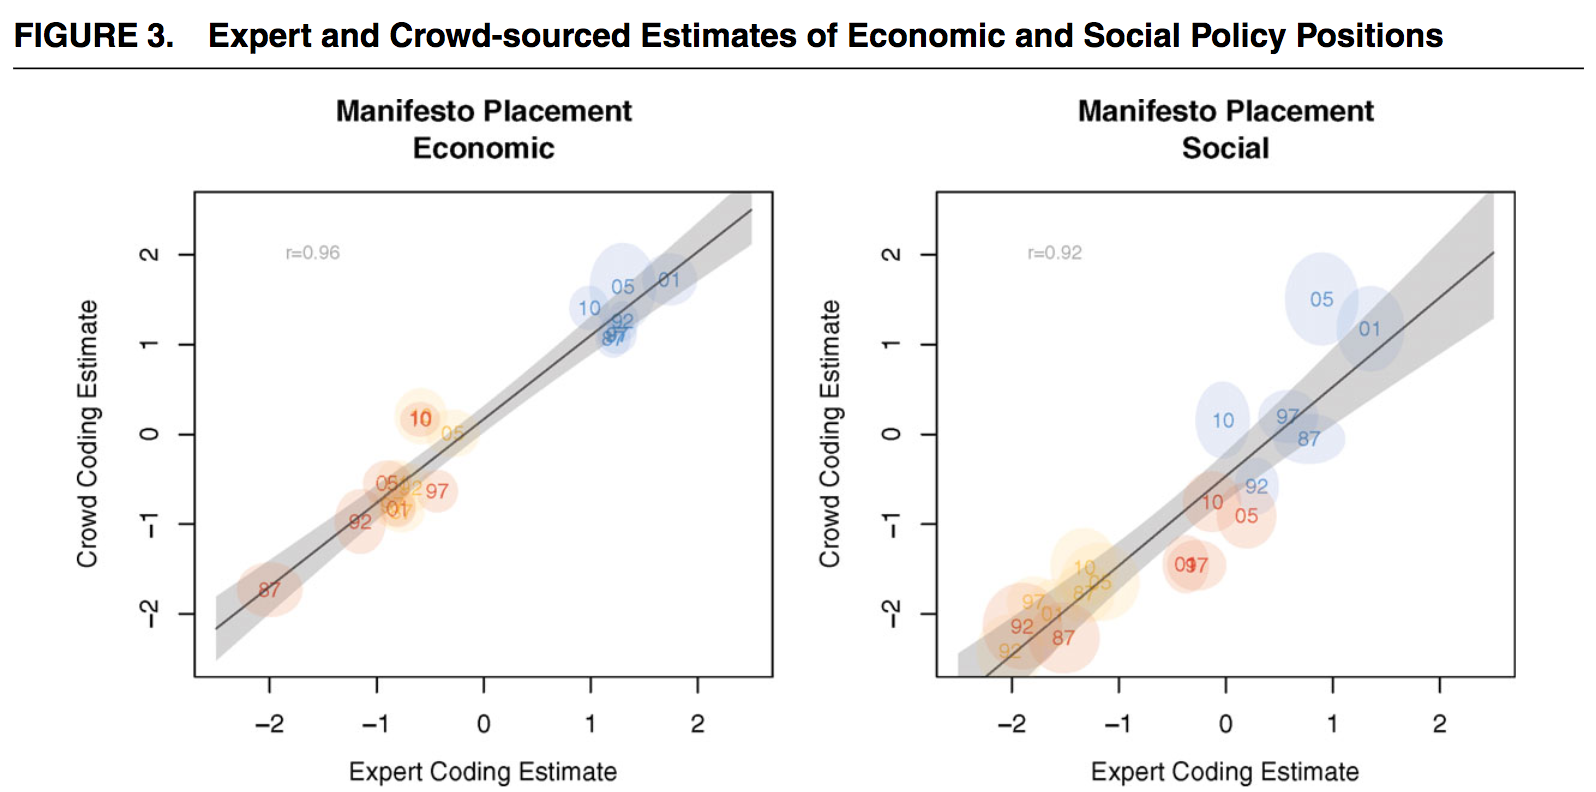
\includegraphics[width=\textwidth]{figures/benoit_crowd-sourced_2016_fig3}}
\end{center}

\end{frame}
%%%%%%%%%%%%%%%%%%%%%%%%%%
\begin{frame}

What I like about Benoit et al (2016)
\begin{itemize}
\item Better not cheaper
\pause
\item Experts are a bug not a feature
\end{itemize}

\end{frame}
%%%%%%%%%%%%%%%%%%%%%%%%%%
\begin{frame}

{\Large
\begin{center}
Questions?
\end{center}
}

\end{frame}
%%%%%%%%%%%%%%%%%%%%%%%%%%
\begin{frame}

\begin{itemize}
\item Human computation
\item \textcolor{blue}{Open call}
\item Distributed data collection
\end{itemize}

\end{frame}
%%%%%%%%%%%%%%%%%%%%%%%%%%
\begin{frame}

\begin{center}
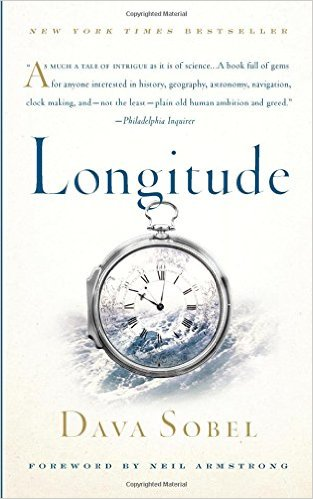
\includegraphics[width=0.3\textwidth]{figures/sobel_longitude_2007_cover}
\end{center}

\end{frame}
%%%%%%%%%%%%%%%%%%%%%%%%%%
\begin{frame}

{\Large
\begin{center}
Solutions are easier to check than to generate
\end{center}
}

\end{frame}
%%%%%%%%%%%%%%%%%%%%%%%%%%
\begin{frame}

{\Large
\begin{center}
You will participate in an open call in a few moments
\end{center}
}

\end{frame}
%%%%%%%%%%%%%%%%%%%%%%%%%%
\begin{frame}

{\Large
\begin{center}
Questions? 
\end{center}
}

\end{frame}
%%%%%%%%%%%%%%%%%%%%%%%%%%
\begin{frame}

\begin{itemize}
\item Human computation
\item Open call
\item \textcolor{blue}{Distributed data collection}
\end{itemize}

\end{frame}
%%%%%%%%%%%%%%%%%%%%%%%%%%
\begin{frame}

\begin{itemize}
\item people can be where the researchers can't
\pause
\item scale that researcher cannot match
\pause
\item sometimes hard to separate from human computation
\end{itemize}

\end{frame}
%%%%%%%%%%%%%%%%%%%%%%%%%%
\begin{frame}

\begin{center}
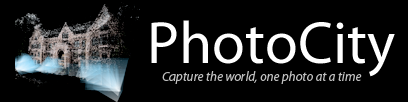
\includegraphics[width=0.6\textwidth]{figures/photocity_logo}
\end{center}

\small{
Tuite et al. (2011) ``PhotoCity: Training Experts at Large-scale Image Acquisition Through a Competitive Game'' \textit{CHI}:  \url{http://dx.doi.org/10.1145/1978942.1979146}
}

\end{frame}
%%%%%%%%%%%%%%%%%%%%
\begin{frame}

\begin{center}
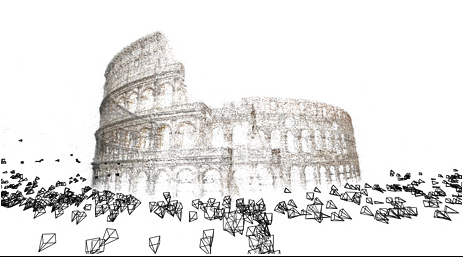
\includegraphics[width=0.6\textwidth]{figures/rome_in_a_day}
\end{center}
Rome in a Day (Agarwal et al., 2009)

\end{frame}
%%%%%%%%%%%%%%%%%
\begin{frame}

\begin{center}
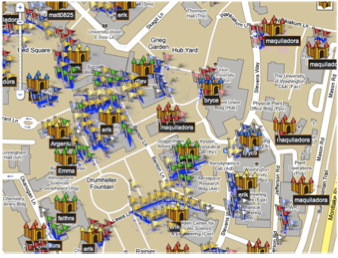
\includegraphics[width=0.6\textwidth]{figures/tuite_photocity_2011_fig2}
\end{center}

Two campuses: University of Washington and Cornell University

\end{frame}
%%%%%%%%%%%%%%%%%
\begin{frame}

Over 2 months, 100,000 photos submitted by 45 players
\vfill
\begin{center}
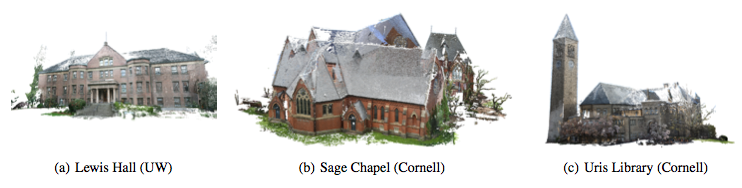
\includegraphics[width=0.9\textwidth]{figures/tuite_photocity_2011_fig8}
\end{center}

\end{frame}
%%%%%%%%%%%%%%%%%
\begin{frame}
\frametitle{PhotoCity}

Beautiful design solves lots of problems
\pause
\begin{itemize}
\item data collection is standardized because of cameras
\pause
\item verification is automatic by comparison with nearby images
\pause
\item game points are assigned based on the value of data, trains people to collect more valuable data
\end{itemize}

\end{frame}
%%%%%%%%%%%%%%%%%%%%%%%%%%
\begin{frame}

{\Large
\begin{center}
Questions about distributed data collection or mass collaboration?
\end{center}
}

\end{frame}
%%%%%%%%%%%%%%%%%%%%%%%%%%

\end{document}
